% This template has been downloaded from:
% http://www.latextemplates.com
%
% Original author:
% Ted Pavlic (http://www.tedpavlic.com)
%
% Modified by:
% Charles Newey (http://assemblyco.de)
%----------------------------------------

% Declare document
\documentclass{article}

% Packages
\usepackage{fancyhdr} % Required for custom headers
\usepackage{lastpage} % Required to determine the last page for the footer
\usepackage{extramarks} % Required for headers and footers
\usepackage{graphicx} % Images
\usepackage{tabularx} % Tables
\usepackage[table]{xcolor} % Table colours
\usepackage[colorlinks]{hyperref} % For URLs
\usepackage[T1]{fontenc} % Support symbols like < and >
\usepackage{lmodern} % Format symbols properly

% Colours
\definecolor{negligible}{rgb}{0.55, 0.71, 0.0}
\definecolor{acute}{rgb}{1.0, 0.75, 0.0}
\definecolor{severe}{rgb}{1.0, 0.49, 0.0}
\definecolor{critical}{rgb}{0.9, 0.17, 0.31}

% Margins
\topmargin=-0.45in
\evensidemargin=0in
\oddsidemargin=0in
\textwidth=6.5in
\textheight=9.0in
\headsep=0.25in
\linespread{1} % Line spacing

% Other setup
\pagestyle{fancy}
\renewcommand\headrulewidth{0.4pt} % Size of the header rule
\renewcommand\footrulewidth{0.4pt} % Size of the footer rule
\setlength\parindent{0pt} % Removes all indentation from paragraphs
\renewcommand{\refname}{} % Removes bibliography title

% Set up constants
\newcommand{\address}{
\small{
	\begin{tabular}{ l}
		Department of Computer Science, \\
		Llandinam Building, \\
		Aberystwyth University, \\
		Aberystwyth, \\
		Ceredigion, \\
		SY23 3DB \\
	\end{tabular}
	}
}

% Set up the header and footer
\lhead{\doctitle}										% Top left header
\chead{\version}										% Top center head
\rhead{\firstxmark \status}								% Top right header
\lfoot{\lastxmark \qanumber}							% Bottom left footer
\cfoot{Aberystwyth University/Computer Science}			% Bottom center footer
\rfoot{Page\ \thepage\ of\ \protect\pageref{LastPage}}	% Bottom right footer

% Set up title page
\title{
	\vspace{1.2in}
	\textmd{\textbf{\doctitle}} \\
	\vspace{0.1in}\large{\textit{\today}} \\
	\vspace{0.4in}
	{\bf{\qanumber}} \\ \vspace{0.4in}
	\version \\
	\status \\
	\vspace{0.4in}
}

\author{\authors}
\date{}


%----------------------------- UPDATE THESE FOR EACH DOCUMENT ------------------------------
\newcommand{\version}{Version: 1.0} %======================================================= DOC VERSION
\newcommand{\status}{Status: Release} %===================================================== DOC STATUS
\newcommand{\qanumber}{SE.10.TEMPLATE.1} %================================================== QA NUMBER
\newcommand{\doctitle}{Group 10 Document Template} %======================================== DOC TITLE

%----------------------------- UPDATE THESE FOR EACH DOCUMENT ------------------------------
%=========================================================================================== VERSION HISTORY
\newcommand{\versionhistory}{
		\begin{tabularx}{\linewidth}{| p{2cm} | p{2cm} | p{2cm} | X | }
			\hline
			\bf{Author} & \bf{Date} & \bf{Version} & \bf{Change made} \\
			\hline
			CCN & 07/11/2013 & 1.1 & Updated order of authors on cover \\
			\hline
			DEC & 07/11/2013 & 1.2 & Added High Level Architecture diagram \\
			\hline
		\end{tabularx}
}

%---------------------------- UPDATE THESE FOR EACH DOCUMENT ------------------------------
%=========================================================================================== AUTHOR LIST
\newcommand{\authors}{
	\begin{tabular}{| l | l |}
		\hline
		\bf{Contributor Name} & \bf{Role} \\
		\hline
		Daniel Clark & Project Lead \\
		\hline
		Mark Lewis & QA Manager \\
		\hline
		Charles Newey & Deputy Project Lead \& Android Developer \\
		\hline
		Martin Ferris & Android Developer \\
		\hline
		Ashley Iles & Android Developer \\
		\hline
		Kenny Packer & Android Developer \\
		\hline
		Stephen McFarlane & Deputy QA \& Web Developer \\
		\hline
		Kieran Palmer & Web Developer \\
		\hline
	\end{tabular}
	% Don't edit this
	\\ \\ \\ \\ \\ \\
	\address \vline
	\hspace{0.15in} \copyright Copyright Group 10, 2013
	% Don't edit this
}

% Make title page, ToC and other introductory elements
\begin{document}
	\maketitle
	\newpage
	\tableofcontents
	\newpage

	% Begin the actual document
	%======================================================================================= DOCUMENT STARTS HERE
	\begin{section}{INTRODUCTION}
		\begin{subsection}{Purpose of This Document}
			The purpose of this document is to show that we have met the outlined objectives specified by the client.
		\end{subsection}
	
		\begin{subsection}{Scope}
			Scope
		\end{subsection}
		
		\begin{subsection}{Objectives}
			\begin{itemize}
				\item{Objective 1}
				\item{Objective 2}
			\end{itemize}
		\end{subsection}
	\end{section}
	
	\newpage
	\begin{section}{SAMPLE IMAGE}
		\begin{center}
		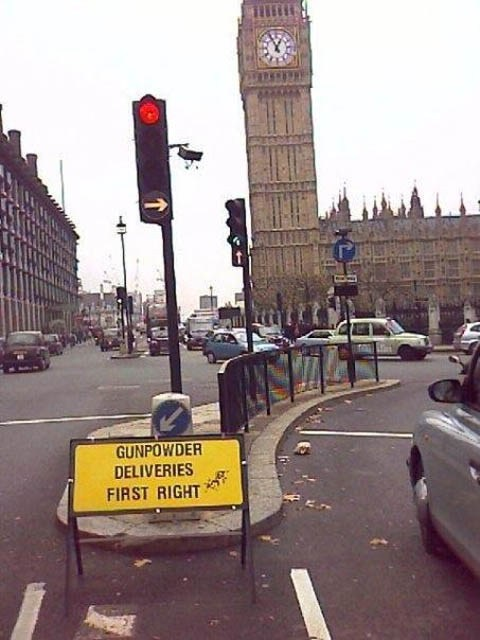
\includegraphics[height=1\columnwidth, angle=90]{images/test.jpg}
		\end{center}
	\end{section}

	% Include references here (edit the References.bib file)
	\nocite{LaTeXTemplate} % DO NOT EDIT

	% Format bibliography/refs
	\newpage
	\begin{section}{REFERENCES}
		\bibliographystyle{acm}
		\bibliography{References}
	\end{section}
	
	\vspace{1cm}
	\begin{section}{VERSION HISTORY}
		\versionhistory
	\end{section}
\end{document}

%									Useful bits and pieces
%\begin{section}{section_name}								% Start section
%\end{section}												% End section
%\begin{center} \end{center}								% Center stuff
%\includegraphics[width=0.75\columnwidth]{example_figure}	% Insert image
%\pseudocode{filename}{caption}								% Insert highlighted code snippet
%\clearpage													% Clear page after section
%\url{http://www.google.com/} 								% Include URL
%\nocite{citationName}										% Cite to bibliography (but not to text)
%\cite{citationName}										% Include reference